\chapter{Progettazione}
Prima di passare alla parte di scrittura del codice si deve decidere "cosa" dovrà fare il codice e come sarà strutturata l'anima dell'applicazione.

\section{Preparazione}
Convalidata l’idea, sono state selezionate le “features” che l’applicazione avrebbe dovuto avere sulla base delle risposte ai sondaggi somministrati agli studenti dei principali atenei di Roma. Il target sarebbe stato un pubblico giovane con bisogni precisi e su di essi è stata costruita la struttura dell’applicazione, tenendo conto delle linee guida della programmazione AGILE, partendo dal modello UML.
Sono state scelte le tecnologie da utilizzare in funzione del tipo di servizio offerto: si è optato per una applicazione mobile Android abbinata ad un server gestito da Microsoft Azure.
Lo sviluppo del progetto è stato suddiviso tra i membri del team per competenze riguardanti i linguaggi di programmazione, tra lato client (Android) e lato server (ASP.Net) , in modo tale da velocizzare il lavoro annullando il tempo di apprendimento di una nuova tecnologia.
Il workshop ci ha fornito la possibilità di lavorare come una squadra per il raggiungimento di un obbiettivo comune e concreto, mettendoci nella condizione di procedere ad un buon ritmo di lavoro, ma soprattutto ci ha dato l’opportunità di iniziare un fondamentale accrescimento personale, fornendoci gli strumenti necessari, accademici e non, in vista di future attività lavorative grazie ad una vera e propria simulazione di progetto aziendale.

\section{Modello UML}
In ingegneria del software, UML (unified modeling language, "linguaggio di modellizzazione unificato") è un linguaggio di modellazione e specifica basato sul paradigma orientato agli oggetti. Il linguaggio nacque con l'intento di unificare approcci precedenti, raccogliendo le migliori prassi nel settore e definendo così uno standard industriale unificato.
UML svolge un'importantissima funzione di "lingua franca" nella comunità della progettazione e programmazione a oggetti. Gran parte della letteratura di settore usa UML per descrivere soluzioni analitiche e progettuali in modo sintetico e comprensibile a un vasto pubblico.
La notazione UML è semi-grafica e semi-formale; un modello UML è costituito da una collezione organizzata di diagrammi correlati, costruiti componendo elementi grafici ed elementi testuali.
Per questo progetto sono state utilizzate due implementazioni di tale linguaggio: il class diagram, necessario per esplicitare il rapporto tra i vari Models ovvero le classi che compongono l'applicazione, e l’ use case diagram, necessario per mostrare il “workflow” dell’interazione tra utente e applicazione.

\subsection{Diagramma delle classi}
Il diagramma delle classi è uno dei tipi di diagrammi del modello UML. Il suo scopo è di rendere visiva l’interazione tra le entità che popoleranno il programma finale. Le relazioni che connettono i modelli rappresentano i legami tra di essi e possono essere accompagnate da ulteriori informazioni, ruolo e molteplicità, per specificare al meglio i vari vincoli.
Ad esempio, nel caso specifico, le due connessioni che collegano il modello Studente con il modello Path mostrano come uno studente possa far parte di molteplici “percorsi” e esserne creatore di altrettanti, ma un percorso può avere un solo creatore. 
La figura  \ref{fig:uml} mostra il digramma completo.

\subsection{Diagramma dei casi d'uso}
Il diagramma dei casi d’uso si occupa invece della descrizione delle funzioni del sistema dal punto di vista degli attori che interagiscono con esso. Questo tipo di diagramma può essere considerato come uno strumento per la rappresentazione dei requisiti funzionali del sistema poiché evidenzia le operazioni che l’utente (Studente) può effettuare (Figura \ref{fig:use-case}).
I "casi" di questo diagramma verranno poi implementati come funzioni che l'applicazione dovrà eseguire.
Le linee in grassetto indicano le operazioni base che l'utente puo compiere.
Tra le varie operazioni possono esistere delle relazioni: <include> indica che l'operazione alla base della freccia è eseguita dopo (o in contemporanea) l'operazione che si trova all'altro capo, mentre <extend> indica che l'operazione alla base della freccia aggiunge funzionalità all'operazione verso cui punta la freccia stessa.
Come possiamo notare, infatti, tutte le operazioni richiedono che l'utente effettui la procedura di login prima di essere eseguite (<include>) mentre l'operazione di "join" aggiunge una funzionalità alla ricerca di un percorso (<extend>).

\begin{figure}[!hb]
  \centering
    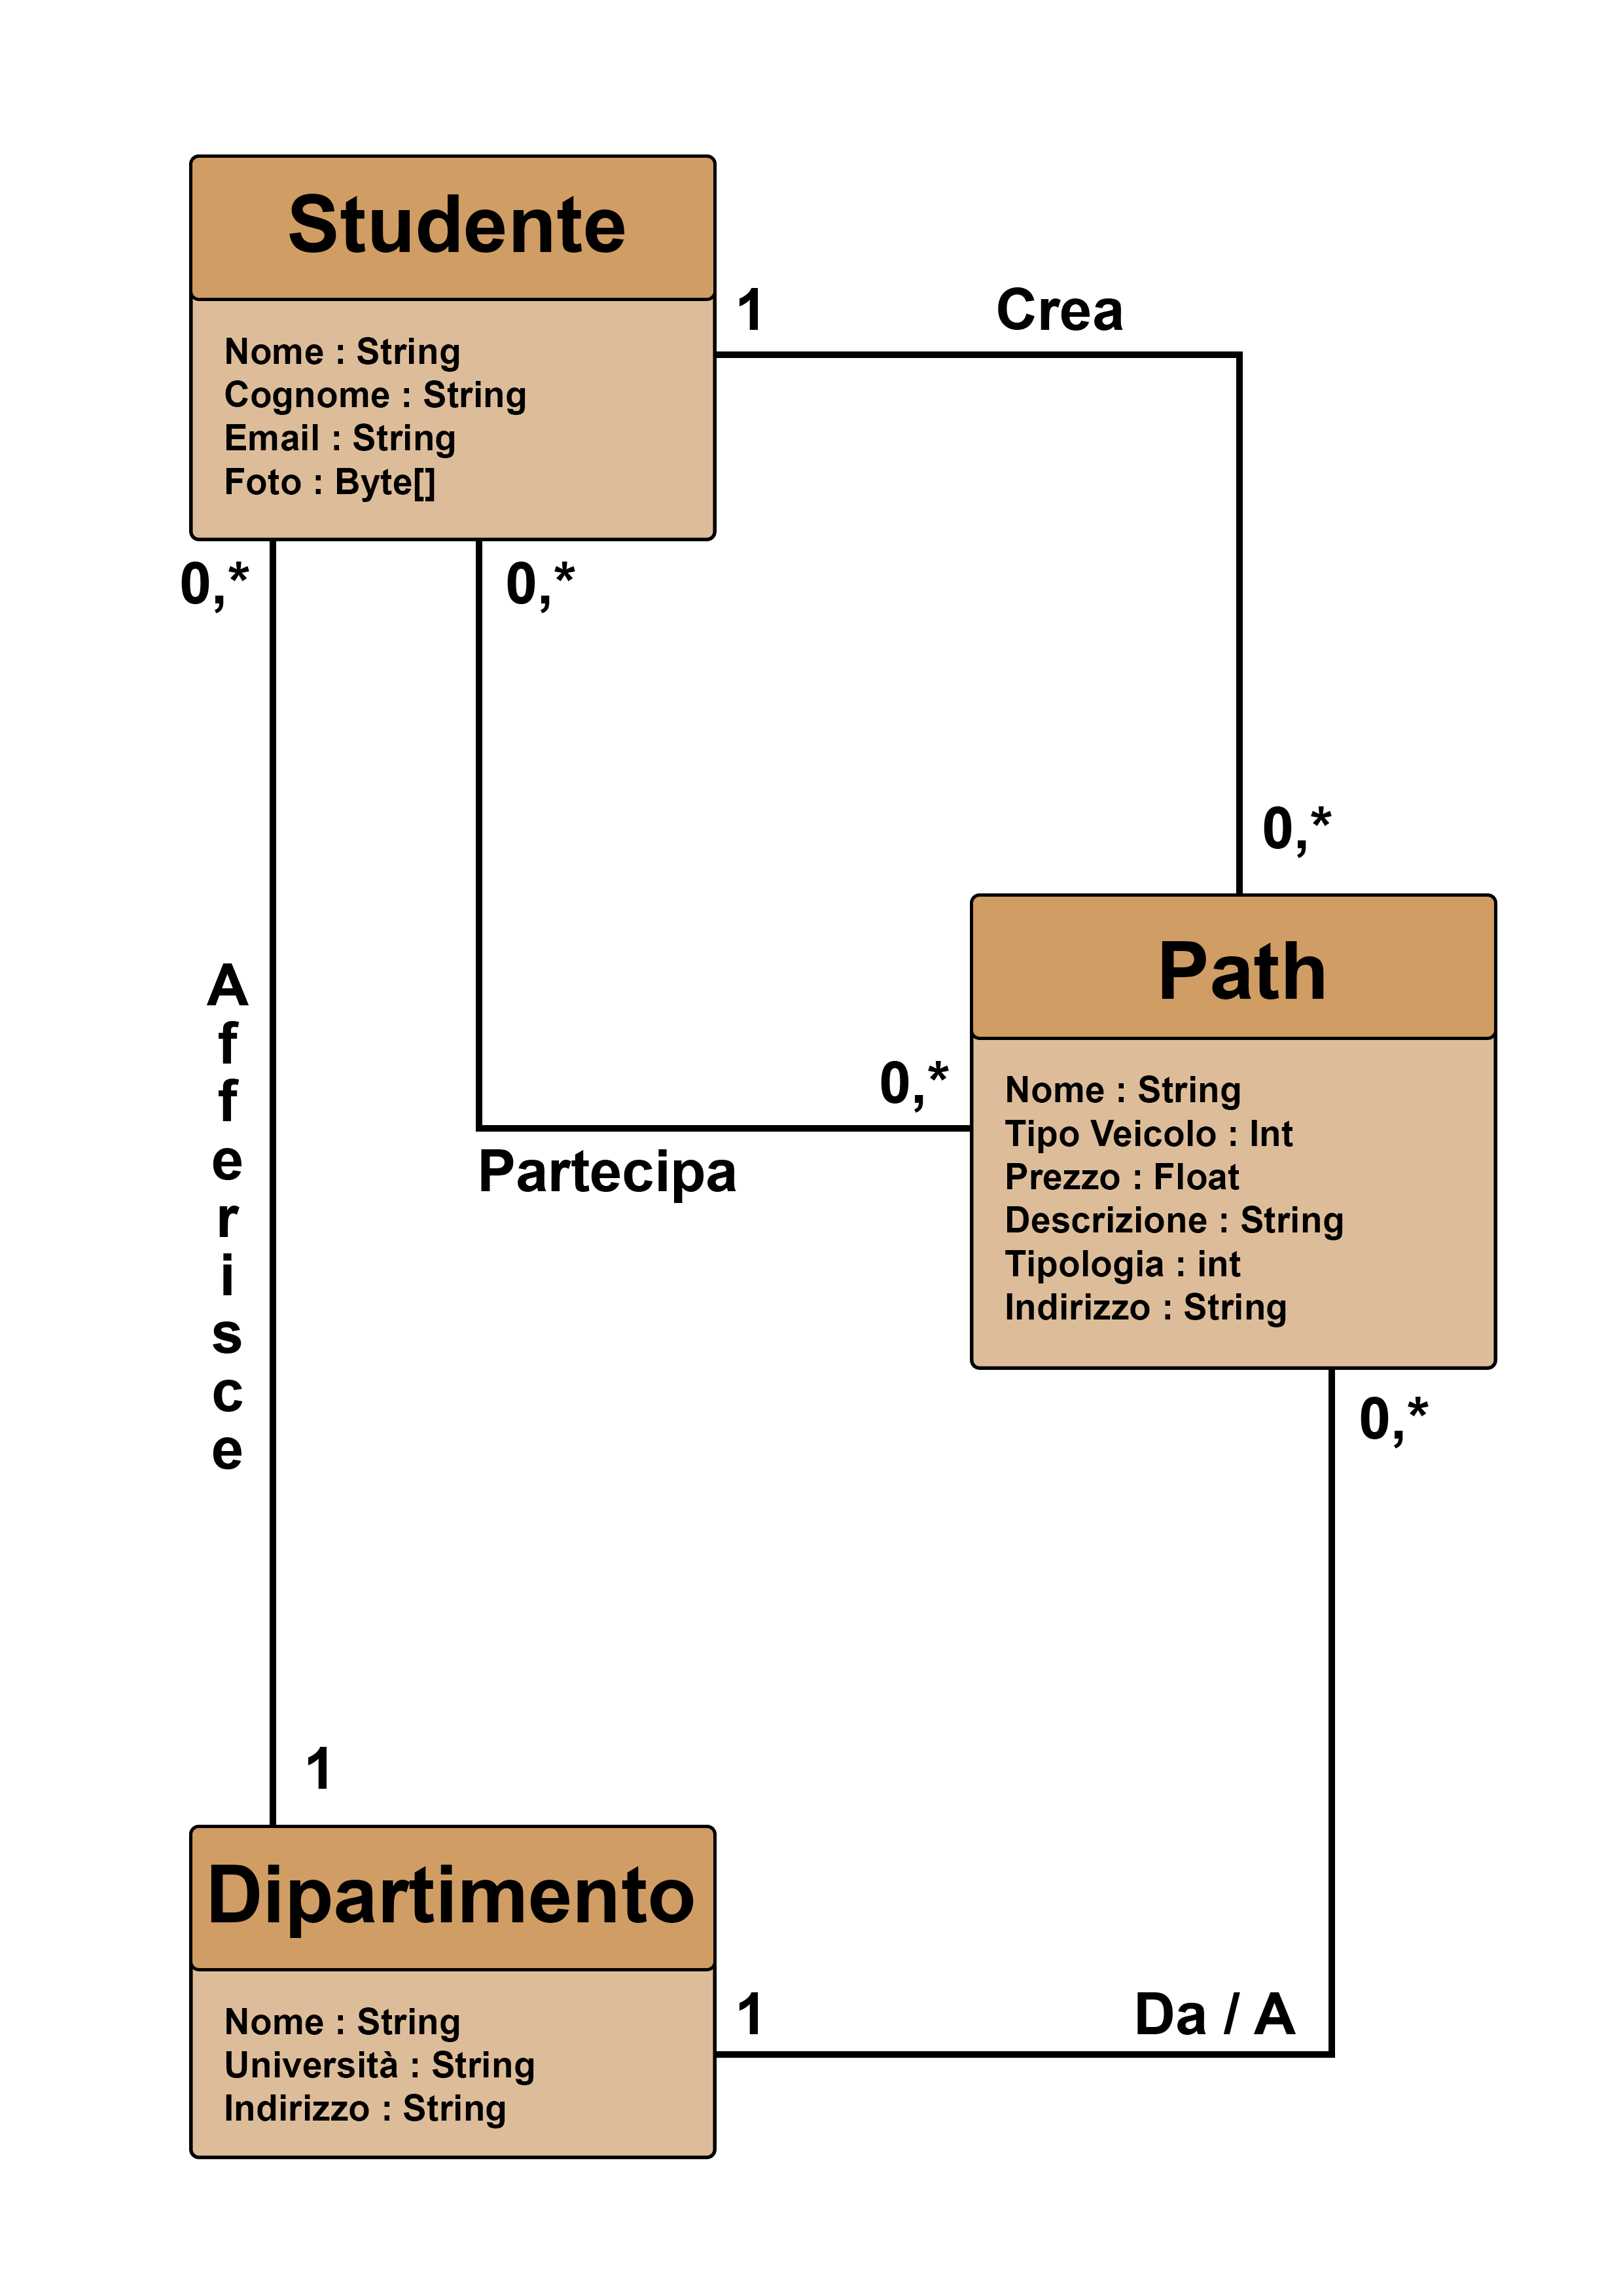
\includegraphics[width=1\textwidth]{uml}
  \caption{Diagramma delle classi}
  \label{fig:uml}
\end{figure}

\begin{figure}[!hb]
  \centering
    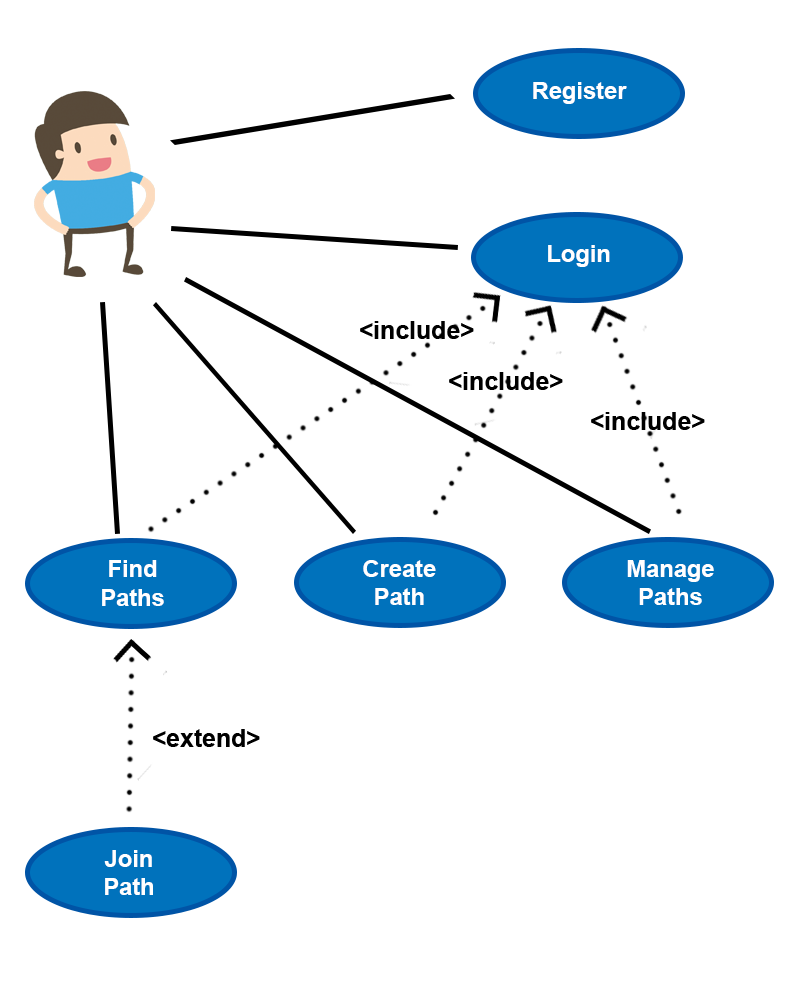
\includegraphics[width=1\textwidth]{use-case}
  \caption{Diagramma dei casi d'uso}
  \label{fig:use-case}
\end{figure}